\PassOptionsToPackage{xcolor}{usenames,dvipsnames,svgnames,table}
\documentclass[10pt]{report}
\usepackage[T1]{fontenc}
\usepackage{lmodern}
\usepackage{pdfcolmk}
\usepackage{multirow}
\usepackage{graphicx}
\usepackage{pifont}
\usepackage{amsmath,amsfonts,amsthm,amssymb}
\usepackage{setspace}
\usepackage{Tabbing}
\usepackage{etoolbox}
\usepackage{fancyhdr}
\usepackage{lastpage}
\usepackage{listings}
\usepackage{extramarks}
\usepackage{enumerate}
\usepackage{soul,color}
\usepackage{graphicx,float,wrapfig}
\usepackage{amsmath,amssymb,rotating}
\usepackage{epsfig}
\usepackage{color}
\usepackage{hyperref}
\usepackage{animate}
\usepackage{array}
\usepackage{graphics, color}
\usepackage{graphicx}
\usepackage{epsfig}
\usepackage{setspace}
\usepackage{verbatim}
\usepackage[margin=1.0in]{geometry}
\usepackage{tikz}
\usepackage{mdframed}
\usepackage{clrscode3e}
\usepackage{formalHW}
\usepackage[imouzon,none]{formatHW}
\usepackage{fancyquote}
\usepackage{fancyenvironments}
\usepackage{mymathmacros}
\usepackage{algorithm}
\usepackage[noend]{algpseudocode}
\usepackage{pgfplots}

%set up fancy page header
\pagestyle{fancy}
         \lhead{\href{mailto:imouzon@iastate.edu}{\nolinkurl{imouzon@iastate.edu}}}
            \lhead{imouzon}
      \chead{\ (,\ ): Sim Cats}  
   \rhead{\firstxmark}
   \lfoot{\lastxmark}
   \cfoot{}
   \rfoot{Page\ \thepage\ of\ \pageref{LastPage}}
   \renewcommand\headrulewidth{0.4pt}
   \renewcommand\footrulewidth{0.4pt}

% pandoc syntax highlighting
\usepackage{color}
\usepackage{fancyvrb}
\newcommand{\VerbBar}{|}
\newcommand{\VERB}{\Verb[commandchars=\\\{\}]}
\DefineVerbatimEnvironment{Highlighting}{Verbatim}{commandchars=\\\{\}}
% Add ',fontsize=\small' for more characters per line
\newenvironment{Shaded}{}{}
\newcommand{\KeywordTok}[1]{\textcolor[rgb]{0.00,0.44,0.13}{\textbf{{#1}}}}
\newcommand{\DataTypeTok}[1]{\textcolor[rgb]{0.56,0.13,0.00}{{#1}}}
\newcommand{\DecValTok}[1]{\textcolor[rgb]{0.25,0.63,0.44}{{#1}}}
\newcommand{\BaseNTok}[1]{\textcolor[rgb]{0.25,0.63,0.44}{{#1}}}
\newcommand{\FloatTok}[1]{\textcolor[rgb]{0.25,0.63,0.44}{{#1}}}
\newcommand{\CharTok}[1]{\textcolor[rgb]{0.25,0.44,0.63}{{#1}}}
\newcommand{\StringTok}[1]{\textcolor[rgb]{0.25,0.44,0.63}{{#1}}}
\newcommand{\CommentTok}[1]{\textcolor[rgb]{0.38,0.63,0.69}{\textit{{#1}}}}
\newcommand{\OtherTok}[1]{\textcolor[rgb]{0.00,0.44,0.13}{{#1}}}
\newcommand{\AlertTok}[1]{\textcolor[rgb]{1.00,0.00,0.00}{\textbf{{#1}}}}
\newcommand{\FunctionTok}[1]{\textcolor[rgb]{0.02,0.16,0.49}{{#1}}}
\newcommand{\RegionMarkerTok}[1]{{#1}}
\newcommand{\ErrorTok}[1]{\textcolor[rgb]{1.00,0.00,0.00}{\textbf{{#1}}}}
\newcommand{\NormalTok}[1]{{#1}}

% header includes

\begin{document}

\thispagestyle{empty}%
\begin{center}%
    \renewcommand{\arraystretch}{1.5}%
    \begin{tabular}{c}%
       \Large{: }\\
       Coupon Similarity Cluster Categories\\
         \\
    \end{tabular}
\end{center}

\begin{center}
 \renewcommand{\arraystretch}{1.5}
 \begin{tabular*}{0.65\textwidth}{r@{:\hspace{.3cm}}l}
    \hline
     Name& Ian Mouzon\\
     email& \href{mailto:imouzon@iastate.edu}{\nolinkurl{imouzon@iastate.edu}}\\
    
    
    
    \hline
 \end{tabular*}
\end{center}

I am using the following packages:

\begin{Shaded}
\begin{Highlighting}[]
   \KeywordTok{library}\NormalTok{(ggplot2)}
   \KeywordTok{library}\NormalTok{(lubridate)}
   \KeywordTok{library}\NormalTok{(xtable)}
   \KeywordTok{library}\NormalTok{(foreach)}
   \KeywordTok{library}\NormalTok{(rCharts)}
   \KeywordTok{library}\NormalTok{(magrittr)}
   \KeywordTok{library}\NormalTok{(tidyr)}
   \KeywordTok{library}\NormalTok{(dplyr)}
   \KeywordTok{library}\NormalTok{(reshape2)}
   \KeywordTok{library}\NormalTok{(gtools)}
   \KeywordTok{library}\NormalTok{(sqldf)}
   \KeywordTok{library}\NormalTok{(missForest)}
   \KeywordTok{source}\NormalTok{(}\StringTok{"./R/renm.R"}\NormalTok{)}
\end{Highlighting}
\end{Shaded}

and our working directory is set to \verb!dmc2015/ian!.

\textbf{Getting the Data and Manipulations}

I am using our new clean data - so should you

\begin{Shaded}
\begin{Highlighting}[]
   \NormalTok{d =}\StringTok{ }\KeywordTok{readRDS}\NormalTok{(}\StringTok{"~/dmc2015/data/clean_data/universalCleanData.rds"}\NormalTok{)}
\end{Highlighting}
\end{Shaded}

I can melt the columns by coupon using the following:

\begin{Shaded}
\begin{Highlighting}[]
\KeywordTok{source}\NormalTok{(}\StringTok{"~/dmc2015/ian/r/stackCoupons2.R"}\NormalTok{)}
\NormalTok{dm =}\StringTok{ }\KeywordTok{stackCoupons2}\NormalTok{(d, }\DataTypeTok{idcols =} \KeywordTok{c}\NormalTok{(}\DecValTok{1}\NormalTok{:}\DecValTok{4}\NormalTok{, }\DecValTok{32}\NormalTok{:}\DecValTok{49}\NormalTok{))}
\end{Highlighting}
\end{Shaded}

I and can split the columns of product group using:

\begin{Shaded}
\begin{Highlighting}[]
\KeywordTok{source}\NormalTok{(}\StringTok{"~/dmc2015/ian/r/splitColumn.R"}\NormalTok{)}
\NormalTok{dmc =}\StringTok{ }\KeywordTok{splitColumn}\NormalTok{(dm, }\StringTok{"categoryIDs"}\NormalTok{, }\StringTok{"orderID"}\NormalTok{, }\DataTypeTok{splitby =} \StringTok{":"}\NormalTok{)}
\end{Highlighting}
\end{Shaded}

\begin{verbatim}
## Loading required package: tcltk
\end{verbatim}

\section{Creating the Item ID}\label{creating-the-item-id}

\begin{Shaded}
\begin{Highlighting}[]
\NormalTok{d$item_id1 =}\StringTok{ }\KeywordTok{with}\NormalTok{(d, }\KeywordTok{paste}\NormalTok{(brand1, productGroup1, categoryIDs1, }\DataTypeTok{sep =} \StringTok{"|"}\NormalTok{))}
\NormalTok{d$item_id2 =}\StringTok{ }\KeywordTok{with}\NormalTok{(d, }\KeywordTok{paste}\NormalTok{(brand2, productGroup2, categoryIDs2, }\DataTypeTok{sep =} \StringTok{"|"}\NormalTok{))}
\NormalTok{d$item_id3 =}\StringTok{ }\KeywordTok{with}\NormalTok{(d, }\KeywordTok{paste}\NormalTok{(brand3, productGroup3, categoryIDs3, }\DataTypeTok{sep =} \StringTok{"|"}\NormalTok{))}
\end{Highlighting}
\end{Shaded}

\subsection{Creating order\_match
class}\label{creating-orderux5fmatch-class}

\begin{Shaded}
\begin{Highlighting}[]
\NormalTok{d$order_match_class =}\StringTok{ }\KeywordTok{factor}\NormalTok{(}\StringTok{"000"}\NormalTok{, }\DataTypeTok{levels =} \KeywordTok{c}\NormalTok{(}\StringTok{"111"}\NormalTok{, }\StringTok{"110"}\NormalTok{, }\StringTok{"101"}\NormalTok{, }\StringTok{"011"}\NormalTok{, }\StringTok{"000"}\NormalTok{))}
\NormalTok{d$order_match_class[(d$item_id1 !=}\StringTok{ }\NormalTok{d$item_id2 &}\StringTok{ }\NormalTok{d$item_id2 ==}\StringTok{ }\NormalTok{d$item_id3)] =}\StringTok{ "011"}
\NormalTok{d$order_match_class[(d$item_id1 !=}\StringTok{ }\NormalTok{d$item_id2 &}\StringTok{ }\NormalTok{d$item_id1 ==}\StringTok{ }\NormalTok{d$item_id3)] =}\StringTok{ "101"}
\NormalTok{d$order_match_class[(d$item_id1 ==}\StringTok{ }\NormalTok{d$item_id2 &}\StringTok{ }\NormalTok{d$item_id1 !=}\StringTok{ }\NormalTok{d$item_id3)] =}\StringTok{ "110"}
\NormalTok{d$order_match_class[(d$item_id1 ==}\StringTok{ }\NormalTok{d$item_id2 &}\StringTok{ }\NormalTok{d$item_id1 ==}\StringTok{ }\NormalTok{d$item_id3)] =}\StringTok{ "111"}
\end{Highlighting}
\end{Shaded}

\subsection{Save the category feature}\label{save-the-category-feature}

\begin{Shaded}
\begin{Highlighting}[]
\NormalTok{d %>%}\StringTok{ }\KeywordTok{select}\NormalTok{(orderID, order_match_class) %>%}\StringTok{ }\KeywordTok{saveRDS}\NormalTok{(}\DataTypeTok{file =} \StringTok{"~/dmc2015/features/feature_files/universal/order_match_class.rds"}\NormalTok{)}
\end{Highlighting}
\end{Shaded}

\section{Results}\label{results}

\begin{Shaded}
\begin{Highlighting}[]
\NormalTok{chk =}\StringTok{ }\NormalTok{d %>%}\StringTok{ }\KeywordTok{mutate}\NormalTok{(}\DataTypeTok{order_res_paste =} \KeywordTok{paste0}\NormalTok{(coupon1Used, coupon2Used, coupon3Used), }
    \DataTypeTok{nCouponUsed =} \NormalTok{coupon1Used +}\StringTok{ }\NormalTok{coupon2Used +}\StringTok{ }\NormalTok{coupon3Used) %>%}\StringTok{ }\KeywordTok{select}\NormalTok{(order_res_paste, }
    \NormalTok{coupon1Used, coupon2Used, coupon3Used, nCouponUsed, order_match_class) %>%}\StringTok{ }
\StringTok{    }\KeywordTok{gather}\NormalTok{(tmp, couponUsed, -order_res_paste, -order_match_class, -nCouponUsed) %>%}\StringTok{ }
\StringTok{    }\KeywordTok{mutate}\NormalTok{(}\DataTypeTok{couponCol =} \KeywordTok{as.numeric}\NormalTok{(}\KeywordTok{gsub}\NormalTok{(}\StringTok{"coupon"}\NormalTok{, }\StringTok{""}\NormalTok{, }\KeywordTok{gsub}\NormalTok{(}\StringTok{"Used"}\NormalTok{, }\StringTok{""}\NormalTok{, tmp)))) %>%}\StringTok{ }
\StringTok{    }\KeywordTok{select}\NormalTok{(-tmp) %>%}\StringTok{ }\KeywordTok{filter}\NormalTok{(order_res_paste !=}\StringTok{ "NANANA"}\NormalTok{)}

\KeywordTok{summary}\NormalTok{(chk$order_match_class)}
\end{Highlighting}
\end{Shaded}

\begin{verbatim}
##   111   110   101   011   000 
##    69   225    69   420 17376
\end{verbatim}

\begin{Shaded}
\begin{Highlighting}[]
\NormalTok{chk$couponMatch =}\StringTok{ }\DecValTok{0}
\NormalTok{for (i in }\DecValTok{1}\NormalTok{:}\KeywordTok{nrow}\NormalTok{(chk)) chk$couponMatch[i] =}\StringTok{ }\DecValTok{1} \NormalTok{*}\StringTok{ }\NormalTok{(}\KeywordTok{as.numeric}\NormalTok{(}\KeywordTok{unlist}\NormalTok{(}\KeywordTok{strsplit}\NormalTok{(}\KeywordTok{as.character}\NormalTok{(chk$order_match_class[i]), }
    \StringTok{""}\NormalTok{))[chk$couponCol[i]]) ==}\StringTok{ }\NormalTok{chk$couponUsed[i])}

\KeywordTok{ggplot}\NormalTok{(}\DataTypeTok{data =} \NormalTok{chk, }\KeywordTok{aes}\NormalTok{(}\DataTypeTok{x =} \NormalTok{order_match_class, }\DataTypeTok{fill =} \NormalTok{couponMatch)) +}\StringTok{ }\KeywordTok{geom_bar}\NormalTok{() +}\StringTok{ }
\StringTok{    }\KeywordTok{facet_grid}\NormalTok{(couponCol ~}\StringTok{ }\NormalTok{couponUsed)}
\end{Highlighting}
\end{Shaded}

\begin{center}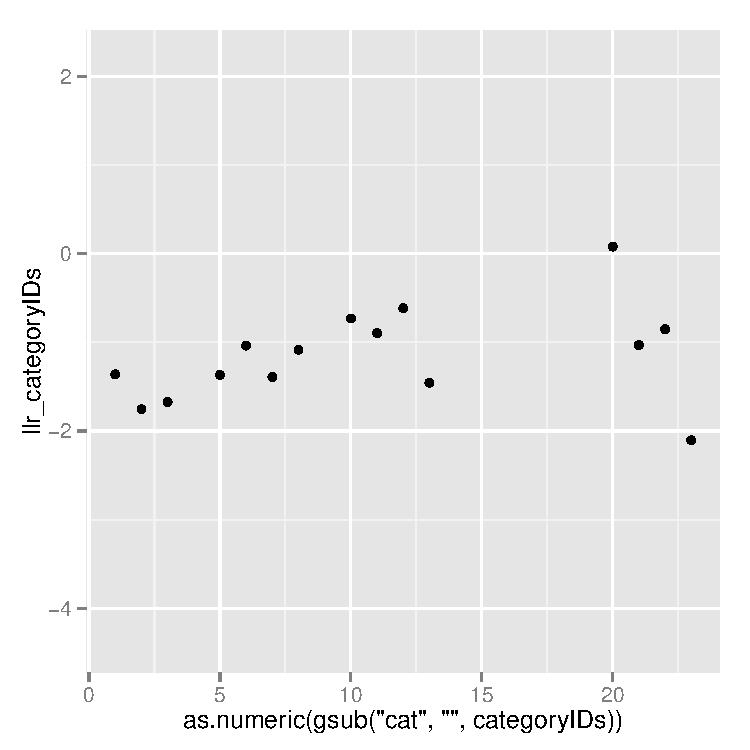
\includegraphics{/Users/user/dmc2015/ian/graphics/fig_unnamed-chunk-6-1} \end{center}

\end{document}
